\chapter{Exercise 07}
\extitle{Practicing Logistic Regression}
%%******************************************************************************%
%                                                                              %
%                                 Interlude                                    %
%                         for Machine Learning module                          %
%                                                                              %
%******************************************************************************%

% =============================================== %
\section*{Interlude - Introducing Polynomial Models}
% ----------------------------------------------- %

You probably noticed that the method we use is called \textit{linear regression} for a reason:
the model generates all of its predictions on a straight line.
However, we often encounter features that do not have a linear relationship with the predicted variable,
like in the figure below:

\begin{figure}[!h]
    \centering
    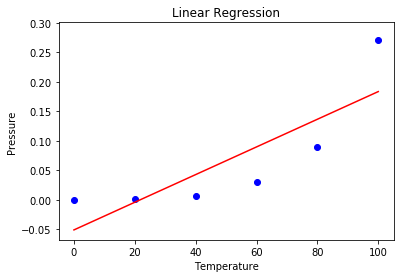
\includegraphics[scale=0.6]{assets/polynomial_straight_line.png}
    \caption{Non-linear relationship}
\end{figure}

In that case, we are stuck with a straight line that cannot fit the data points properly.
In this example, what if we could express $y$ not as a function of $x$, but also of $x^2$, and maybe even $x^3$ and $x^4$?
We could make a hypothesis that draws a nice \textbf{curve} that would better fit the data.
That's where polynomial features can help!

% =============================================== %
\section*{Interlude - Polynomial features}
% ----------------------------------------------- %
First we get to do some \textit{feature engineering}.
We create new features by raising our initial $x$ feature to the power of 2, and then 3, 4... as far as we want to go.
For each new feature we need to create a new column in the dataset.

% =============================================== %
\section*{Interlude - Polynomial Hypothesis}
% ----------------------------------------------- %
Now that we created our new features, we can combine them in a linear hypothesis that looks just the same as what we're used to:

$$
\hat{y} = \theta_0 + \theta_1 x  +\theta_2 x^{2} + \dots + \theta_n x^{n}
$$  

It's a little strange because we are building a linear combination, not with different features but with different powers of the same feature.
This is a first way of introducing non-linearity in a regression model!
%\newpage
\turnindir{ex07}
\exnumber{07}
\exfiles{mono\_log.py, multi\_log.py}
\exforbidden{sklearn}
\makeheaderfilesforbidden


% ================================= %
\section*{Objective}
% --------------------------------- %
Now it's time to test your Logistic Regression Classifier on real data!\\
\\ 
To do so, you will use the \textbf{solar\_system\_census\_dataset}.

% ================================= %
\section*{Instructions}
% --------------------------------- %
Some words about the dataset:
\begin{itemize}
  \item You will work with data from the last Solar System Census.
  \item The dataset is divided in two files which can be found in the \texttt{resources} folder: \texttt{solar\_system\_census.csv} and \texttt{solar\_system\_census\_planets.csv}.
  \item The first file contains biometric information such as the height, weight, and bone density of several Solar System citizens.
  \item The second file contains the home planet of each citizen, indicated by its Space Zipcode representation (i.e. one number for each planet... :)).
\end{itemize}

\newpage
As you should know, Solar citizens come from four registered areas (zipcodes): 
\begin{itemize}
  \item The flying cities of Venus (0)
  \item United Nations of Earth (1)
  \item Mars Republic (2)
  \item The Asteroids' Belt colonies (3)
\end{itemize}
\bigskip
You are expected to produce 2 programs that will use Logistic Regression to predict which planet 
each citizen comes from, based on the other variables found in the census dataset.\\
\\
But wait... what? There are four different planets! How do you make a classifier 
discriminate between 4 categories?!!\\
\\
Keep calm and take a sip of water, we'll go one step at the time ...\\

% ================================= %
\subsection*{One Label to Discriminate Them All}
% --------------------------------- %
You already wrote a Logistic Regression Classifier that can discriminate between two classes. We can use it 
to solve this problem!\\
\\
Let's start by having it discriminate between citizens who come from your favorite planet and everybody else!\\
\\
Your program (in \texttt{mono\_log.py}) will:
\begin{enumerate}
  \item Take an argument: \texttt{--zipcode=x} with $x$ being $0$, $1$, $2$ or $3$.
        If no argument, usage will be displayed.
  \item Split the dataset into a training and a test set.
  \item Select your favorite Space Zipcode and generate a new \texttt{numpy.array} to label each citizen according to your new selection criterion:
  \begin{itemize}
    \item $1$ if the citizen's zipcode corresponds to your favorite planet.
    \item $0$ if the citizen has another zipcode.
  \end{itemize}
  \item Train a logistic model to predict if a citizen comes from your favorite planet or not, using your brand new label.
  \item Calculate and display the fraction of correct predictions over the total number of predictions based on the test set.
  \item Plot 3 scatter plots (one for each pair of citizen features) with the dataset and the final prediction of the model.
\end{enumerate}
\hint{You can use normalization on your dataset but the question is ... Should you?}
\noindent{You now have a model that can discriminate between citizens that come 
from one specific planet and everyone else.}\\
\\
It's a first step, and a good one, but we still have work to do before we can classify citizens 
among the four planets of our dataset!\\
\\
So how does \textbf{Multiclass Logistic Regression} work?\\
% ================================= %
\subsection*{One Versus All}
% --------------------------------- %
The idea now is to apply what is called \textbf{one-versus-all classification}. 
As you will see, this is quite straightforward.\\
\\
Your program (in \texttt{multi\_log.py}) will:
\begin{enumerate}
  \item Split the dataset into a training and a test set.
  \item Train 4 logistic regression classifiers to discriminate each class 
  from the others (the way you did in part one).
  \item Predict for each example the class according to each classifier and
   select the one with the highest output probability score.
  \item Calculate and display the fraction of correct predictions over the 
  total number of predictions based on the test set.
  \item Plot 3 scatter plots (one for each pair of citizen features) with the
   dataset and the final prediction of the model.
\end{enumerate}

% ================================= %
\section*{Examples}
% --------------------------------- %
If a cititzen got the following classification probabilities: 
\begin{itemize}
  \item Planet 0 vs all: $0.38$
  \item Planet 1 vs all: $0.51$
  \item Planet 2 vs all: $0.12$
  \item Planet 3 vs all: $0.89$
\end{itemize}

Then the citizen should be classified as coming from \textit{Planet 3}. 